\documentclass[platex]{suribt}
\usepackage{url}
\usepackage{graphicx}
\usepackage[dvipdfmx]{color}
\usepackage{here}
\usepackage{amsmath}
\title{ランダムフォレストによるサッカーW杯の優勝国予想}
\author{石田亜斗武}
\eauthor{Atomu Ishida}% Copyright 表示で使われる
\studentid{2014011}
\supervisor{六井 淳 教授\deputy 渡邊貴之 教授}% 1 つ引数をとる (役職まで含めて書く)
\handin{2024}{1}% 提出月. 2 つ (年, 月) 引数をとる

\begin{document}
\maketitle%%%%%%%%%%%%%%%%%%% タイトル %%%%


\frontmatter% ここから前文
\begin{jabstract}%%%%%%%%%%%%% 概要 %%%%%%%%
  スポーツの勝敗予測は、選手のコンディション、戦術の変化、チームの相互作用など、多数の変数に影響される。本研究では、私自身の長年のサッカーの経験と、人工知能や機械学習の知識を使い、FIFAワールドカップ優勝国の予測を行う。\par
  本研究ではスポーツの勝敗予測における変数の複雑性に対応するため、ランダムフォレストという機械学習手法を用いる。ランダムフォレストはモデル構築とチューニングの容易さから、活用範囲の広い手法であることが知られている。FIFAワールドカップの優勝国を予測するために過去の大会の結果からデータセットを作成し、ランダムフォレストで予測モデルを構築し予測を行った。

\end{jabstract}

\newpage


\begin{eabstract}%%%%%%%%%%%%% 概要 %%%%%%%%
  Predicting winners and losers in sports is extremely difficult because it is influenced by numerous variables, such as player conditions, tactical changes, and team interactions. In recent years, statistical methods and machine learning have been used to improve the accuracy of predicting the outcome of difficult-to-predict sports matches. Therefore, in this study, I will use my own many years of soccer experience and knowledge of artificial intelligence and machine learning to predict the FIFA World Cup winning country.\par
  To cope with the complexity of variables in sports win/loss prediction, this study uses a machine learning method called random forests. Compared to other methods, Random Forest captures the diversity and complexity of the data by utilizing a large number of decision trees, reducing the risk of overlearning and providing reliable prediction results. In addition, it is easy to build and tune models, enabling results to be achieved within a limited research timeframe. The results of this research are expected to provide useful information for those involved in the FIFA World Cup in response to the growing use of data in the field of sports analysis. 
\end{eabstract}

\setcounter{tocdepth}{2}
\tableofcontents%%%%%%%%%%%%% 目次 %%%%%%%%
\listoffigures%%%%%%%%%%%%% 図目次 %%%%%%%%
\listoftables%%%%%%%%%%%%% 表目次 %%%%%%%%

\mainmatter% ここから本文 %%% 本文 %%%%%%%%
\chapter{はじめに}
\section{研究背景}
スポーツの勝敗予測は、選手のコンディション、戦術の変化、チームの相互作用など、多数の変数に影響されるため、予測が非常に困難である[1]。近年では、予測が困難なスポーツの試合結果を科学的に分析するアナリティクスの分野が注目され、予測の精度を高めるために統計的手法や機械学習が利用されるようになっている[2]。本研究では、私自身の長年のサッカーの経験と、人工知能や機械学習の知識を使い、FIFAワールドカップ優勝国の予測を行う。
\section{研究目的}
本研究の目的は、過去のFIFAワールドカップのデータをもとに高精度な予測モデルを構築し、優勝国を予測することである。サッカーの試合結果予測においては、様々な機械学習手法が採用されている。イングランドのプロサッカーリーグの試合結果予測を行った研究[3]では、決定木[4]によってデータの特徴間の関係をモデル化しやすくし、ナイーブベイズ[5]によって特徴間の独立性を仮定することで、サッカーのような多くの変数が影響するデータに対応し予測を行っている。また同じくイングランドのプロサッカーリーグに対して試合結果予測を行った別の研究[6]では、サポートベクタマシン[7]の過学習[8]を防ぎながら限られたデータからでも高い予測精度を達成するという特性を活かして予測を行っている。\par

本研究ではこれらの手法の中からランダムフォレスト[9]を採用する。ランダムフォレストは、複数の決定木を組み合わせることでデータの多様性と複雑な関連性を捉え、過学習のリスクを減らすことができる[10][11]ため、ナイーブベイズの変数同士の複雑な関係やデータパターンを捉えるのには限界があるという欠点[12]を解決することでき、決定木の訓練データに過剰に適合する傾向がある[13]という問題を解決することができる。また、ランダムフォレストにはモデル構築とチューニングの容易であるという特徴があり[14]、サポートベクタマシンのモデル設計やチューニングが困難であるという欠点[15]を解決することができる。\par

さらに、本研究ではランダムフォレストを用いた先行研究[16][17]では取り扱わないジニ係数[18]を特徴量としてを加える。ジニ係数とは国の貧富格差を示す指標であり、貧困がサッカーにおけるスキルの習得と知覚運動スキルの発達にプラスの影響を与えるといった研究[19]もある。これは、従来のサッカーの勝敗予測ではあまり注目されてこなかった選手の心理的側面を考慮することにより、試合結果に影響を与える可能性のある新たな要因をモデルに組み込む試みである。このアプローチにより、単に試合結果の統計的な情報だけでなく、選手の心理状態も試合結果予測の重要な要素として取り入れることができると考える。ランダムフォレストを用いたクラス分類によってFIFAワールドカップの優勝国予測を目的とした検証実験を行う。
\section{論文の構成}
第2章では、本研究の関連技術と用語について述べる。\par
第3章では、検証実験について述べる。\par
第4章では、まとめと今後について述べる。

\chapter{関連技術}
本章では、本研究に関連する技術について述べる。
\section{ランダムフォレスト}
ランダムフォレストは、決定木を基にした集団学習アルゴリズムである[20]。この手法では、多数の決定木がデータの異なるランダムなサブセットに基づいて訓練され、それぞれの出力に基づいて最終的な予測結果が多数決または平均値によって決定される(図2.1)。

\begin{figure}[H]
  \centering
  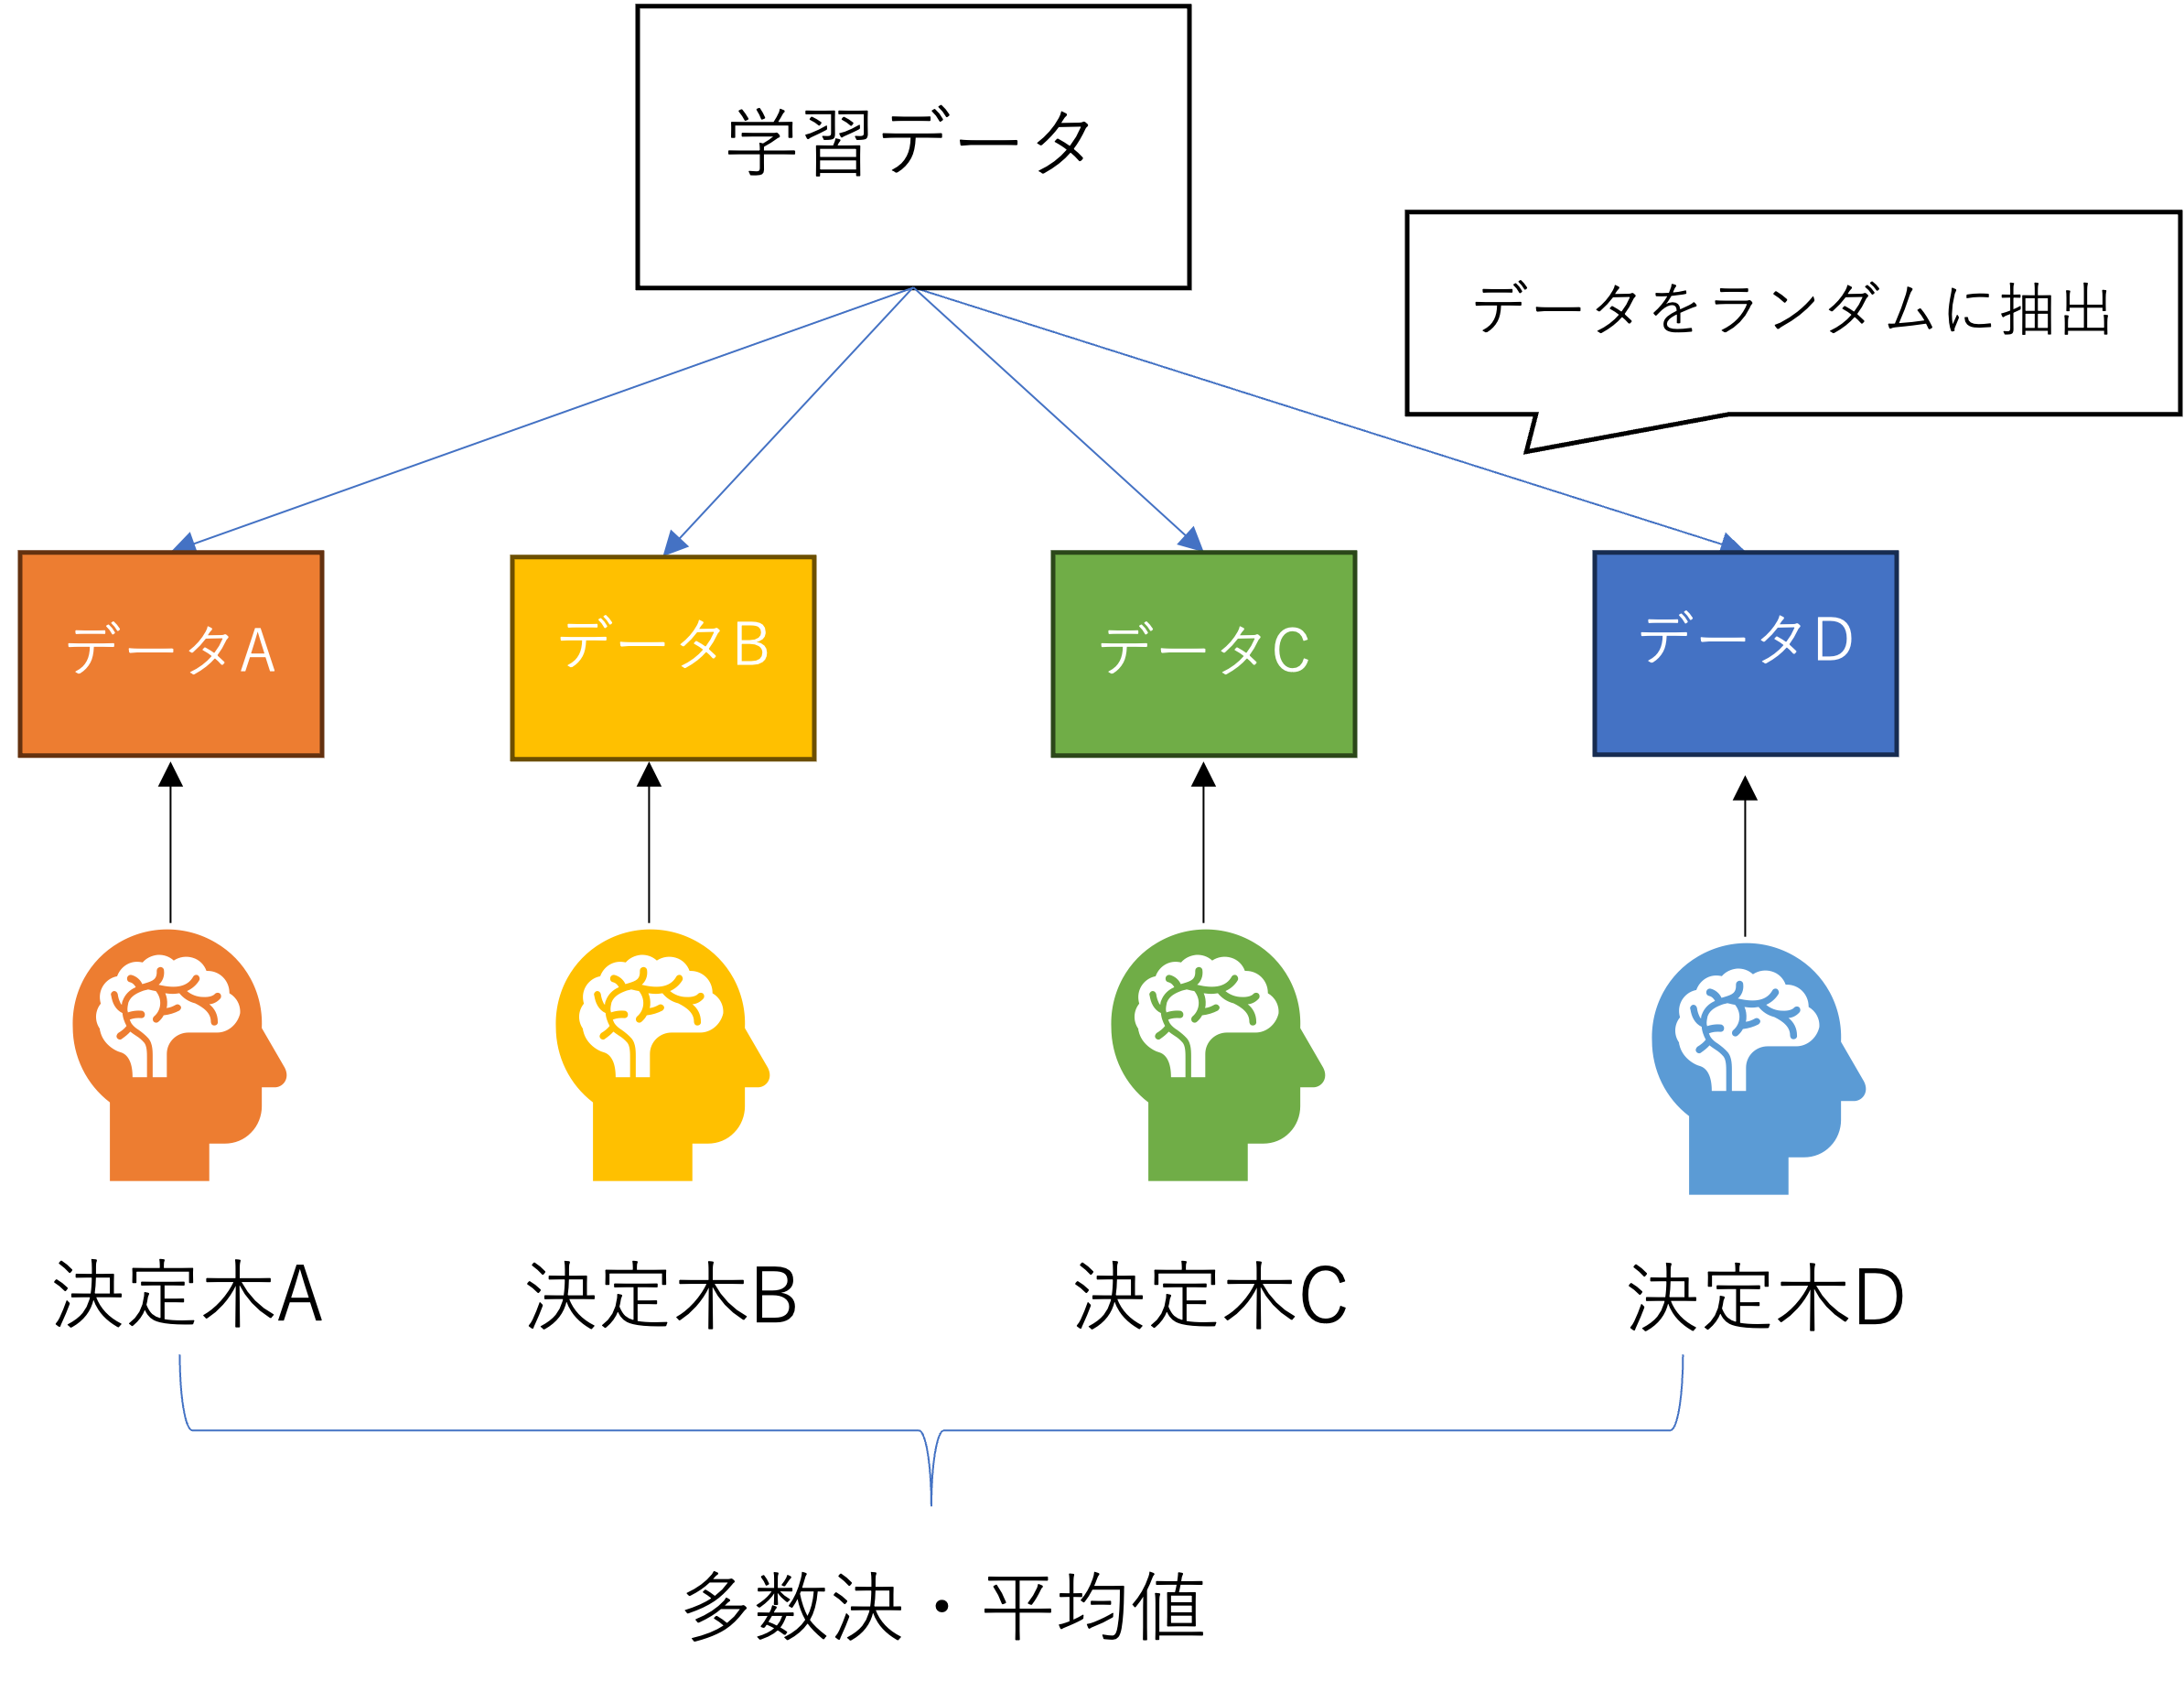
\includegraphics[scale=0.6]{randomforest.png}
  \caption{ランダムフォレストの仕組み}    \label{randomforest}
\end{figure}
  

ランダムフォレストの大きな特徴は、個々の決定木の学習にランダム性を導入している点にある。これによって、各決定木が相補的に機能し、過学習を防ぎつつ高い汎化性能を得ることが可能となる。いかにその流れを説明する[21]。

ランダムフォレストの学習メカニズムは、ランダム性を2つの主要な側面で取り入れる。まず、バギング(Bootstrap Aggregating)[22]を用いて、各決定木の訓練データを選定する。これは、元のデータセット \(S\) から重複を許してランダムにサンプル \(S_{0t}\) を抽出するプロセスである。次に、決定木の各ノードでの分割関数の学習にランダム性を導入する。分割関数のパラメータ \(\theta_j\) に対する候補集合 \(\tau\) は、一般に広範囲にわたるが、そのサブセット \(\tau_j \subseteq \tau\) のみを使用し、その選択をランダムに行う。

ランダム性の度合いは、比率 \(|\tau_j| / |\tau|\) によって調整可能である。ここで、\(\rho = |\tau_j|\) はランダム性の指標として機能し、\(\rho\) の値に応じて、木間の相関が変化する。例えば、\(\rho = |\tau|\) の場合、すべての決定木で同一の学習データが使用されるため、ランダム性はない。逆に、\(\rho = 1\) の場合、完全にランダムな選択が行われ、互いに相関のない決定木が得られる。

各決定木の構築では、根ノードから始めて、最適な分割関数を選択し、データを左右の子ノードに割り当てる。この過程は、すべてのノードにおいて再帰的に繰り返される。具体的には、ノード番号 \(i\) のデータセット \(S_i\) が分割関数によって分割され、左右の子ノードに対応するデータセット \(S_{iL}\) と \(S_{iR}\) に割り当てられる。このプロセスは、決定木のすべてのノードで順に実行され、各ノードで \(S_j = S_{jL} \cup S_{jR}\) および \(S_{jL} \cap S_{jR} = \emptyset\)、\(S_{jL} = S_{2j+1}\)、\(S_{jR} = S_{2j+2}\) が成立する。

分割関数 \(h(v, \theta_j)\) の学習は、ノード \(j\) における最適なパラメータ \(\theta_j^*\) を選択するプロセスであり、式(2.1)のように定義される:
\begin{equation}
\theta_j^* = \arg \max_{\theta_j \in \tau_j} I_j(S_j, S_{jL}, S_{jR}, \theta_j)
\end{equation}
ここで、\(I_j\) は情報利得を表す目的関数である。情報利得は式(2.2)のように計算される:
\begin{equation}
I_j = H(S_j) - \sum_{i \in \{L, R\}} \frac{|S_{ji}|}{|S_j|} H(S_{ji})
\end{equation}
ここで、\(H(S)\) はデータセット \(S\) のエントロピーであり、\(S_{ji}\) はノード \(j\) の左右の子ノードに割り当てられるデータセットを示す。

以上の学習アルゴリズムは、決定木のノードに割り当てられる学習データ集合の数が1になるまで継続される。ただし、過学習を防ぐために適切な停止条件を設定する必要がある。そのための方法としては、あらかじめ設定した最大高さ \(D\) に達した場合、ノードに割り当てられた学習データの個数が一定値以下になった場合、または分割による情報利得が一定値以下になった場合などがある。

\subsection{特徴選択}
ランダムフォレストは特徴量選択をすることで、各決定木でランダムに選択された特徴量のサブセットを使用することで、データセットの異なる側面を捉え、全体としてバランスの取れた分析を行うことができる。本研究で用いるscikit-learnでの分類問題における計算を例に以下に説明する[23]。

特徴量の重要度の計算においてジニ不純度が重要である。ジニ不純度 \( G(k) \) は、特定のノードにおけるサンプルの分布の均一性を測定する。式(2.3)
\begin{equation}
G(k) = \sum_{i=1}^{n} p(i) \times (1-p(i))
\end{equation}
は、ノード \( k \) におけるターゲットラベル \( i \) の出現確率 \( p(i) \) を用いて、そのノードの不純度を算出する。完全に均一なサンプルの集合(すべてが同じラベル)の場合、ジニ不純度は0となり、サンプルが多様なラベルを持つほどジニ不純度は高くなる。

特徴量の重要度 \( I(j) \) は、特徴量がデータの分割にどれだけ効果的に寄与しているかを示す。特徴量 \( j \) を用いてノードを分割することで得られるジニ不純度の減少量を、すべてのノードにわたって集計する。この計算は、式(2.4)
\begin{equation}
\begin{split}
I(j) = \sum_{i=1}^{n \in F(j)} (N_{parent}(i) \times G_{parent}(i)) - (N_{left\*child}(i) \times G*{left\*child}(i) \\ + N*{right\*child}(i) \times G*{right\*child}(i))
\end{split}
\end{equation}
によって表される。ここで、\( F(j) \) は特徴量 \( j \) が分割に使用されるノードの集合を示し、\( N*{parent}(i) \)、\( N_{left\*child}(i) \)、\( N*{right\*child}(i) \) はそれぞれ親ノードとその子ノードのサンプル数を表す。\( G*{parent}(i) \)、\( G_{left\*child}(i) \)、\( G*{right\_child}(i) \) はそれぞれのノードにおけるジニ不純度を示す。

このようにして計算された特徴量の重要度は、モデルにおける各特徴量の寄与度を示し、モデルの解釈に役立つ。特に、予測結果に大きな影響を与える特徴量を特定することで、より効果的な特徴量エンジニアリングやモデルの改善に繋がる。また、データセット内の特徴量間の関係性を理解する上で重要な手がかりを提供する。
\section{データの前処理}
本章では、データの不均衡問題への対策として用いるデータ前処理の技術について述べる。これらの技術は、特に分類問題におけるクラス間の不均衡を解消し、モデルの予測性能を高めるために重要である。データセットにおけるクラス間の不均衡は、分類モデルにおいて重大な課題である[24]。正例(少数クラス)と負例(多数クラス)のデータが不均等である場合、分類モデルは多数クラスの特徴を過剰に学習する傾向があり、少数クラスの重要な特徴を見落とす可能性が高まる。これは、少数クラスの予測精度が著しく低下する結果を招き、誤った結果を導いてしまう可能性がある。
\subsection{アンダーサンプリング}
アンダーサンプリングは、多数クラスのデータをランダムまたは戦略的に減少させる手法であり、データセット内のクラス間のバランスを改善する[25](図2.2)。この手法は、分類モデルが多数クラスに偏らず、少数クラスの特徴を適切に学習する機会を提供する。アンダーサンプリングは、データセットから重要な情報を保持しつつ、クラス間の不均衡を軽減することで、モデルの全体的な分類精度を向上させる効果が期待される。

\begin{figure}[H]
  \centering
  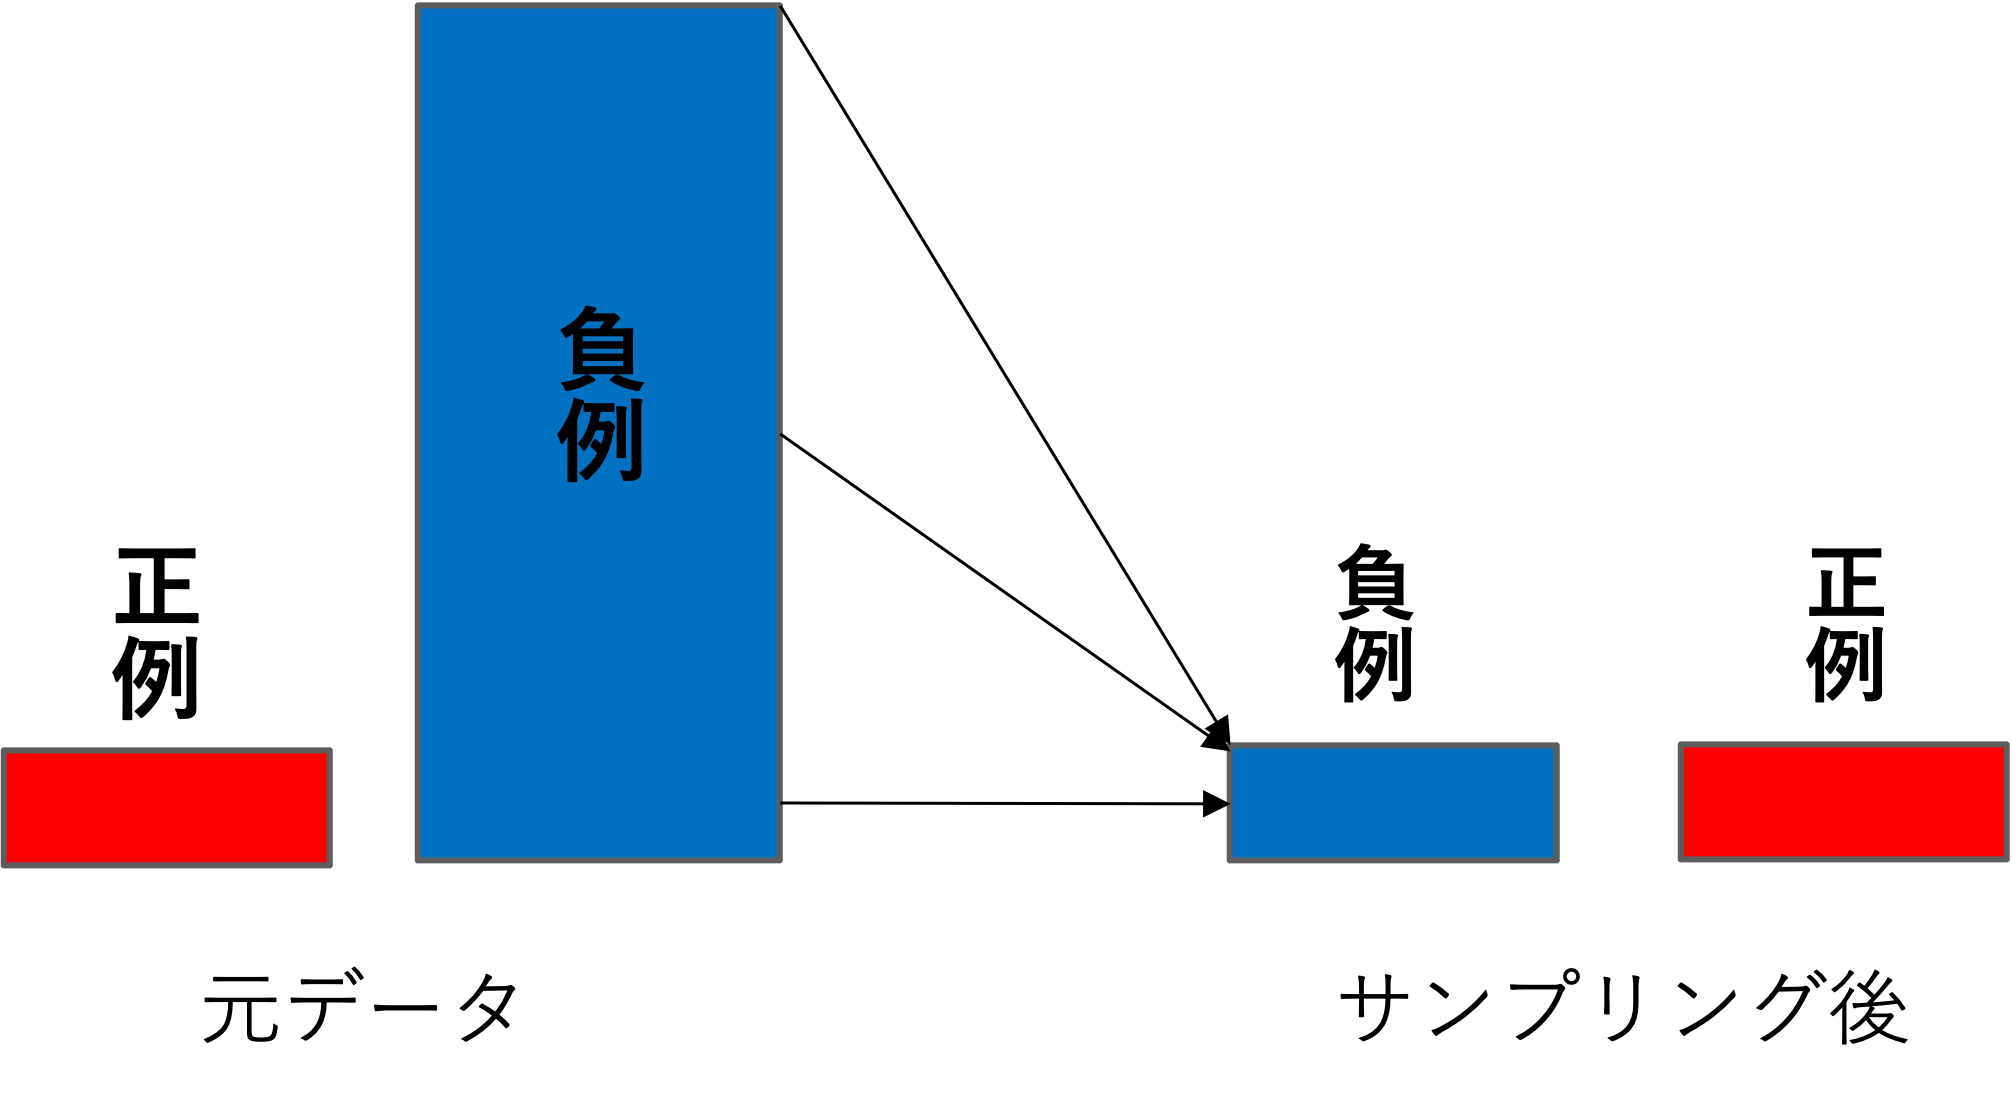
\includegraphics[scale=0.6]{undersampling.png}
  \caption{アンダーサンプリング}    \label{undersampling}
\end{figure}

\subsection{SMOTE}
SMOTE(Synthetic Minority Over-sampling Technique)は、少数クラスの既存サンプルから新たな合成サンプルを生成する手法であり、少数クラスのデータ量を増やすことでデータセットのバランスを改善する[25]。具体的には、SMOTEでは次のステップでサンプルを生成する。

\begin{enumerate}
   \item マイノリティクラスのサンプルからランダムに一つ選択する
   \item 選択したサンプルの最も近い隣人(通常はk-最近傍法により選定)を見つける。
   \item 選択したサンプルとその隣人との間でランダムな点を生成する
\end{enumerate}

このプロセスを繰り返すことで、マイノリティクラスのサンプル数を増やし、データセットのバランスを改善し、モデルが少数クラスの特徴をより深く学習することで偏りのない予測を行えるようにする。SMOTEによって増やされたデータは、モデルのトレーニング中に多様性を提供し、特に少数クラスの識別能力を強化する効果がある。
\subsection{アンダーサンプリングとSMOTEの統合}
本研究では、アンダーサンプリングとSMOTEを組み合わせることで、多数クラスのデータ削減と少数クラスのデータ増加を効果的に行い、クラス間のバランスを適切に調整する。この統合されたアプローチは、分類モデルが全クラスの特徴を均等に学習し、各クラスに対して公平な予測を行うための基盤を提供する。特に、クラス間の不均衡が顕著なデータセットにおいて、この組み合わせはモデルの予測性能の向上に貢献することが期待される。
\section{ハイパーパラメータチューニング}
ハイパーパラメータとは、モデルの学習プロセス中に事前に設定されるパラメータであり、モデルの性能に直接影響を与える。特にランダムフォレストモデルの場合、ハイパーパラメータはモデルの複雑性や学習能力を決定するため、その設定はモデルの成功に不可欠である。ハイパーパラメータの適切な設定は、モデルがデータから複雑なパターンを把握し、予測精度を最大化する上で重要な役割を果たす。これは、モデルがデータをどのように処理し、学習するかを決定するためである。例えば、決定木の数や各木の最大深度は、モデルの複雑さと一般化能力のバランスに影響を与える。過度な複雑さは過学習を引き起こす可能性があり、一方で単純すぎるモデルは未知のデータに対して十分な予測能力を発揮できない。ハイパーパラメータの適切な設定は、モデルの性能を向上させるだけでなく、データの特性や機械学習アルゴリズムの挙動に対する理解を深める効果もある。したがって、ハイパーパラメータの選択とチューニングは、データサイエンスの分野において、効果的なモデル構築に不可欠なスキルであると言える[26]。

ランダムフォレストモデルにおけるハイパーパラメータの適切な設定は、モデルの性能を決定する上で重要な役割を果たす[27]。本研究で用いるscikit-learnのRandomForestClassifierで設定するハイパーパラメータには、決定木の数(n\_estimators)、最大深度(max\_depth)、最小サンプル分割(min\_samples\_split)、最小サンプル葉(min\_samples\_leaf)等がある[28]。決定木の数は、モデルによって生成される決定木の総数を表し、モデルの堅牢性と直接的に関連する。木の数が多ければ多いほど、モデルはより詳細なデータ構造を学習する可能性が高まるが、同時に計算コストも増加する。したがって、モデルの性能と計算効率を考慮して、最適な木の数を決定する必要がある。最大深度は、モデルが学習する際に各決定木が到達することのできる最大の深さを定義する。深い木はより複雑なデータ構造を捉えることができるが、過学習を引き起こすリスクも伴う。適切な最大深度の設定は、モデルが過学習せずにデータを効果的に学習するために重要である。最小サンプル分割は、ノードを分割するために必要な最小サンプル数を指定し、モデルの学習プロセスにおける分割の決定に影響を与える。このパラメータが高い値に設定されると、モデルはデータの小さな変動に対して過敏に反応しなくなり、過学習のリスクが低減される。最小サンプル葉は、葉ノードに存在すべき最小サンプル数を定義する。このパラメータはモデルがデータのノイズに対してどれだけ敏感に反応するかを制御し、特にノイズが多いデータセットにおいて重要である。これらのハイパーパラメータは、モデルの予測精度、訓練時間、複雑性に大きく影響を与える。適切なパラメータの選択により、特定のデータセットに適応した最適なモデルの構築が可能となる。

ランダムフォレストモデルの最適なハイパーパラメータを見つけるためには、効果的なチューニング方法が必要である。主要なチューニング手法にはグリッドサーチとランダムサーチがあり、それぞれが特定の利点を持つ[29]。グリッドサーチは、指定されたハイパーパラメータの全ての組み合わせを網羅的に試す手法である。ハイパーパラメータの候補値をグリッド状に配置し、各組み合わせに対してモデルのパフォーマンスを評価する。この方法の利点は、与えられた値の範囲内で最適な組み合わせを見つける可能性が高いことである。しかし、大きなパラメータ空間を持つモデルでは計算コストが非常に高くなる可能性がある。一方、ランダムサーチは、パラメータ空間内のランダムな点を選択してモデルを評価する手法である。グリッドサーチと比較して、ランダムサーチは計算コストが低く、広範なパラメータ空間の探索が可能である。しかし、ランダム性により、最適なパラメータを見逃す可能性もある。

ハイパーパラメータチューニングは反復的なプロセスであり、異なるパラメータのセットでモデルを評価し、得られた結果を比較して最適な設定を見つける。このプロセスは、モデルの予測性能を最大化し、特定のデータセットに対する最適な適応を実現するために不可欠である。


\chapter{検証実験}
\section{データ詳細}
本研究では、サッカーワールドカップの過去の成績データ、各国のチーム統計データ、国内平均身長、国の経済格差を示すジニ係数などを使用する。これらのデータは、サッカーに関する幅広いデータを提供するデータベースサイトであるSoccer D.B.[31]、世界各国の平均身長や体重に関する情報を提供するウェブサイトであるWorldData.info[32]、世界銀行が提供する公式データベースであるTHE WORLD BANK[33]から収集した。

本研究では、過去のサッカーW杯大会の結果から出場回数、優勝回数、準優勝回数、3位回数、4位回数、試合数、勝利数、引き分け数、敗戦数、勝ち点数、得点数、失点数、開催国等の13種類のデータを使用する。また、各国のチームの統計データとしては、本研究の予測対象であるワールドカップが開催された2014年、2018年、2022年の過去3年間を基準にした国際大会における試合数、平均勝ち点、勝率、得点数、平均得点数、失点数、平均失点数の7種類のデータを用いる。さらに、先行研究[30]から各国のチャンピオンズリーグ出場選手数、五輪出場選手数、FIFAランキング、国内平均身長の4種類のデータも活用する。

さらに重要なデータとしてジニ係数を加える。ジニ係数とは、国の所得分配の不均衡を測る指標で、0(完全な平等)から1(完全な不平等)までの値を取る[18]。ジニ係数を加える決め手として、先行研究[19]から貧困がサッカーにおけるスキルの習得と知覚運動スキルの発達にプラスの影響を与えることが分かっており、従来のサッカーの勝敗予測ではあまり注目されてこなかった選手の心理的側面を考慮することにより、試合結果に影響を与える可能性がある。また、このジニ係数はランダムフォレストアルゴリズムにおける「ジニ不純度」とは異なり、ジニ不純度は決定木の分岐においてデータの均一性を測定するために使用される指標である。
\section{評価指標}
本研究ではデータの分類結果の正解率、適合率、再現率、F値の4つを用いる。
\subsection{混合行列}
混合行列(confusion matrix)は実際のクラス(真の値)と予測されたクラス(予測値)を行と列に持つ表で表現される(図3.1)。二項分類の場合、この行列は4つの異なる領域から成り立つ。
\begin{table}[h]
  \centering
  \begin{tabular}{|l|c|c|}
  \hline
  \multicolumn{1}{|c|}{\textbf{実際のクラス}} & \multicolumn{2}{c|}{\textbf{予測されたクラス}} \\ \hline
   & 正のクラス & 負のクラス \\ \hline
  正のクラス & 真陽性 (TP) & 偽陽性 (FP) \\ \hline
  負のクラス & 偽陰性 (FN) & 真陰性 (TN) \\ \hline
  \end{tabular}
  \caption{混合行列}
\end{table}

ここで、
\begin{itemize}
  \item  真陽性(TP)は正のクラスと正しく予測されたケースの数
  \item  偽陽性(FP)は負のクラスが誤って正と予測されたケースの数
  \item  偽陰性(FN)は正のクラスが誤って負と予測されたケースの数
  \item  真陰性(TN)は負のクラスと正しく予測されたケースの数
\end{itemize}
である。


\subsection{正解率}
正解率(Accuracy)は、「すべての予測のうち、正解した予測の割合」を示し、以下のように計算される。
\begin{equation}
  \text{Accuracy} = \frac{TP + TN}{TP + TN + FP + FN}
\end{equation}

\subsection{適合率}
適合率(precision)とは、陽性と予測された項目の中で実際に陽性である項目の割合を指す。この指標は偽陽性の数を重視する場面で重要であり、偽陽性の増加は適合率の減少をもたらす。適合率の計算式は式(3.2)の通りである。

\begin{equation}
  P = \frac{TP}{TP + FP}
\end{equation}


適合率は、偽陽性(FP)の数を少なく保ちたい場合に用いるべき指標である。誤って陽性と判定してしまうリスクが高い状況でその効果を発揮する。しかし、適合率には陰性の予測を考慮に入れないという弱点がある。偽陰性(FN)が多くても、それは適合率には反映されない。
\subsection{再現率}
再現率(recall)とは、実際に陽性である項目の中で、正しく陽性と予測された項目の割合を示す指標である。偽陰性の数が多いほど再現率は低下するため、実際の陽性を見逃さないようにしたい場面で特に重要である。再現率の計算式は式(3.3)のとおりである。

\begin{equation}
  R = \frac{TP}{TP + FN}
\end{equation}

再現率は、実際の陽性を見逃すことなく特定したいとき、つまり偽陰性(FN)を最小限に抑えたい状況で優先される指標である。例えば医療診断で病気を見逃さないことが重要な場合などが該当する。再現率が高ければ高いほど、少ない見逃しで正確な陽性予測が可能であるが、これは偽陽性の増加を意味する場合もある。
\subsection{F値}
F値(F-measure)とは、適合率と再現率の調和平均である。この指標は、2つの指標のバランスを一つの数値で示すために用いられ、特に両方の性能を同時に考慮する必要がある場合に役立つ。F値は次の式で計算される。

\begin{equation}
F = \frac{2 \times P \times R}{P + R}
\end{equation}

適合率が高いが再現率が低い、あるいはその逆の場合にF値が有用である。F値はこれらの極端なケースを防ぐため、両方の指標を組み合わせたもので、偽陽性と偽陰性の両方を同時に考慮に入れる。
\section{検証内容}
本研究では2010年までのワールドカップデータを活用し、ランダムフォレストアルゴリズムを用いて優勝国の予測モデルを訓練する。訓練データに含まれている各国の過去の成績や統計情報は、モデルが優勝国を予測するためのパターンを学習する基盤となる。特に、各国が準決勝以上に進出するかどうか、そして優勝したかどうかという情報が、分析の主要な焦点である。

本研究では、訓練データとして2010年までのワールドカップデータや各国のチーム統計データ、国内平均身長、国の経済格差を示すジニ係数を扱う。訓練データの前処理として、アンダーサンプリングやSMOTEを組み合わせてクラス間の不均衡を調整し、特徴量選択を行って重要なデータのみを抽出する。さらに、ハイパーパラメータチューニングによりモデルの性能を最適化し、特徴選択によって得られたデータを基に優勝国を予測するためのパターンを学習する。このアプローチにより、準決勝以上に進出する4か国を予測し、その後これらの国々の中から優勝国を予測する。

モデルの検証には2014年、2018年、2022年のワールドカップ結果を使用する。3大会に限定した理由は、これ以上のデータ収集には時間的な制約があるためであり、データの量と質を考慮し、最も効率的かつ現実的な範囲で分析を行うことを目指したためである。使用する評価指標には正解率、適合率、再現率、F1スコアを含み、これによりモデルの予測能力と汎用性を検証する。
\section{検証結果}
\subsection{特徴量選択の結果}
特徴量選択によって選ばれた特徴量は、出場回数、優勝回数、準優勝回数、3位回数、4位回数、試合数、勝利数、引き分け数、勝ち点数、得点数、失点数、過去3年の国際大会の勝率、FIFAランキング、CL出場選手数、ジニ係数の15種類であった。

\subsection{2014年の結果}

2014年の分類結果を表3.2に示す。この結果は、準決勝以上に進む4か国の3か国以上を正確に予測できていることを示しているが、適合率の値が低いため、誤った予測も行っていることが示唆される。

2014年の予測結果を以下の表3.3と表3.4に示す。表3.3では、準決勝以上に進むと予測した国のうち、最も確率の高い4か国を予測結果として示している。
準決勝以上に進む4か国については3か国予測できているが、優勝国であるドイツを予測することができなかった。

\begin{table}[h]
  \centering
  \begin{tabular}{|c|c|c|c|}
    \hline
    正解率 & 適合率 & 再現率 & F値 \\ \hline
    75.6% & 42.9% & 75% & 54.6% \\ \hline
  \end{tabular}
  \caption{2014年の分類結果}
\end{table}

\begin{table}[h]
  \centering
  \begin{tabular}{|c|c|}
    \hline
    予測結果 & 正解 \\ \hline
    スペイン &  ×(アルゼンチン)\\ \hline
    オランダ &  ○ \\ \hline
    ドイツ & ○ \\ \hline
    ブラジル & ○  \\ \hline
  \end{tabular}
  \caption{2014年の準決勝以上に進む国の予測結果}
\end{table}

\begin{table}[h]
  \centering
  \begin{tabular}{|c|c|}
    \hline
    予測結果 & 正解 \\ \hline
    ブラジル & ×(ドイツ) \\ \hline
  \end{tabular}
  \caption{2014年の優勝国の予測結果}
\end{table}

\subsection{2018年の結果}
2018年の分類結果を表3.5に示す。この結果は、準決勝以上に進む4か国のうち1か国しか予測できず、適合率の値も低いため、多くの誤った予測も行っていることが示唆される。

2018年の予測結果を以下の表3.6と表3.7に示す。表3.3では、準決勝以上に進むと予測した国のうち、最も確率の高い4か国を予測結果として示している。
準決勝以上に進む4か国については1か国のみ予測でき、優勝国であるフランスは予測することができなかった。

\begin{table}[h]
  \centering
  \begin{tabular}{|c|c|c|c|}
    \hline
    正解率 & 適合率 & 再現率 & F値 \\ \hline
    61.4% & 16.7% & 25% & 20% \\ \hline
  \end{tabular}
  \caption{2018年の分類結果}
\end{table}

\begin{table}[h]
  \centering
  \begin{tabular}{|c|c|}
    \hline
    予測結果 & 正解 \\ \hline
    ブラジル &  ×(フランス)\\ \hline
    イングランド &  ○ \\ \hline
    アルゼンチン & ×(ベルギー) \\ \hline
    オランダ & ×(クロアチア) \\ \hline
  \end{tabular}
  \caption{2018年の準決勝以上に進む国の予測結果}
\end{table}

\begin{table}[h]
  \centering
  \begin{tabular}{|c|c|}
    \hline
    予測結果 & 正解 \\ \hline
    ブラジル & ×(フランス) \\ \hline
  \end{tabular}
  \caption{2018年の優勝国の予測結果}
\end{table}

\subsection{2022年の結果}
2022年の分類結果を表3.8に示す。この結果は、準決勝以上に進む4か国の半数を正確に予測できていることを示しているが、適合率が低いため、多くの誤った予測も行っていることが示唆される。

2022年の予測結果を以下の表3.9と表3.10に示す。表3.3では、準決勝以上に進むと予測した国のうち、最も確率の高い4か国を予測結果として示している。準決勝以上に進む4か国については2か国予測できているが、優勝国であるアルゼンチンを予測することができなかった。

\begin{table}
  \centering
  \begin{tabular}{|c|c|c|c|}
    \hline
    正解率 & 適合率 & 再現率 & F値 \\ \hline
    67.3% & 33.3% & 50% & 40% \\ \hline
  \end{tabular}
  \caption{2022年の検証結果}
\end{table}

\begin{table}
  \centering
  \begin{tabular}{|c|c|}
    \hline
    予測結果 & 正解 \\ \hline
    フランス & ○ \\ \hline
    アルゼンチン & ○ \\ \hline
    ドイツ & ×(モンゴル) \\ \hline
    ブラジル & ×(クロアチア) \\ \hline
  \end{tabular}
  \caption{2022年の準決勝以上に進む国の予測結果}
\end{table}

\begin{table}
  \centering
  \begin{tabular}{|c|c|}
    \hline
    予測結果 & 正解 \\ \hline
    ドイツ & ×(アルゼンチン) \\ \hline
  \end{tabular}
  \caption{2022年の優勝国の予測結果}
\end{table}

\section{考察}
選択された特徴量には、過去のワールドカップの結果をはじめ、先行研究にはない本研究での取り組みであるジニ係数が選ばれており、従来の特徴量だけでは捉えきれなかった経済的要素が予測モデルに組み込まれ、予測性能が向上した可能性がある。

2014年から2022年の結果を比べると、どの結果も準決勝以上に進む国を1カ国以上は予測できたものの、優勝国は予測することができなかった。また、どの予測結果においてもブラジルやドイツなど過去のワールドカップにおいて優勝経験が多く、優秀な結果を残した国が予測されていることから、2018年や2022年など過去のワールドカップではあまり良い結果を残していない国に対しての予測が難しいことが考えられる。

準決勝以上に進む国に対しては、平均して半分の国を予測することができたが、すべての予測で優勝国を的中させることができなかった。このことから選択された特徴量やモデルが最終的な勝者を決めるキーとなる要素を捉えていないことが明らかになった。優勝国を予測するためには、歴代の優勝国に対するより微細な分析をし、準決勝や決勝で勝利するために重要となる要素の特定が必要である。

\chapter{まとめと今後の課題}

\section{まとめ}
本研究では、ランダムフォレストアルゴリズムを用いてFIFAワールドカップの優勝国を予測するモデルを構築した。使用されたデータセットは、過去のワールドカップ大会の成績、チームの統計データ、サッカー協会のランキング情報、そして各国の経済的、身体的情報といった複数の要素から構成された。特に、ジニ係数という国の経済格差を示す指標を加えることで、従来のサッカーの勝敗予測ではあまり注目されてこなかった選手の心理的側面を考慮し、試合結果に影響を与える可能性のある新たな要因をモデルに組み込む試みを行った。検証結果は過去3大会の準決勝以上に進む国に対しては一定数の予測を行うことができたが、3大会とも優勝国を予測することは出来なかった。
\section{今後の課題}
今後の課題は次のとおりである。

\begin{enumerate}
  \item 特徴量の再評価とバランスの取れた重み付け
  \item 特定試合における勝敗の決定要因の分析
\end{enumerate}



また二つ目の課題については、今回の予測では準決勝以上に進む国に対しては一定以上の予測をすることは出来たが、優勝国を予測することができなかったため、準決勝や決勝といった重要な試合における勝利に影響を与える要素に注目し、それらの要素をモデルに統合することで優勝国に対する予測の精度を高めることができると考える。

\backmatter% ここから後付
\chapter{謝辞}%%%%%%%%%%%%%%% 謝辞 %%%%%%%

本研究を行うにあたり、六井淳教授には指導教員として多くのご助言を賜り、最後までご指導ご鞭撻頂きました。心より御礼申し上げます。また、数々のご協力とご助言を頂いた六井研究室の皆様方、副査の渡辺貴之教授にもこの場をお借りして深く感謝いたします。

\begin{thebibliography}{2}%%%% 参考文献 %%%
\bibitem{}
Milad Keshtkar Langaroudi, Mohammad Reza Yamaghani, “Sports Result Prediction Based on Machine Learning and Computational Intelligence Approaches A Survey”, P1, 2019
\bibitem{}
谷岡広樹, "スポーツアナリティクスにおけるデータとAI活用",P1, 2020
\bibitem{}
Saurabh Vaidya ,”Football Match Winner Prediction”, P1,P2, 2016
\bibitem{}
Lucidspark, "決定木分析とは?メリットとやり方", \url{https://lucidspark.com/ja/blog/how-to-make-a-decision-tree}
\bibitem{}
AVINTON ,”機械学習入門者向け Naive Bayes(単純ベイズ)アルゴリズムに触れてみる”,\url{https://avinton.com/academy/naive-bayes/}
\bibitem{}
Chinwe Peace Igiri,"Support Vector Machine-Based Prediction System for a Football Match Result", P1, 2015
\bibitem{}
AIsmiley, "サポートベクターマシン(SVM)とは?特徴やメリットと活用事例", \url{https://aismiley.co.jp/ai_news/svm/}
\bibitem{}
TRYETING"機械学習における過学習とは何か?原因・回避方法をくわしく解説", \url{https://www.tryeting.jp/column/6846/}
\bibitem{}
IBM"ランダムフォレストとは",\url{https://www.ibm.com/jp-ja/topics/random-forest}
\bibitem{}
Matthias Schonlau, Rosie Yuyan Zou, "The random forest algorithm for statistical learning", P4, 2020
\bibitem{}
Kai Liang,"Analysis and Evaluation of Sports Effect Based on Random Forest Algo-rithm under Big Data",P2, 2022
\bibitem{}
OpenGenus"9Advantages and 10disadvantages of Naive Bayes Algorithm", \url{https://iq.opengenus.org/advantages-and-disadvantages-of-naive-bayes-algorithm/}
\bibitem{}
InsideLearningMachines"8 Key Advantages And Disadvantages Of Decision Trees”, \url{https://insidelearningmachines.com/advantages_and_disadvantages_of_decision_trees/}
\bibitem{}
”Hyperparameters and Tuning Strategies for Random Forest”, \url{https://ar5iv.labs.arxiv.org/html/1804.03515}, 2019
\bibitem{}
Rosita Guido, ”A hyper-parameter tuning approach for cost-sensitive support vector machine classifiers”,P3,2022
\bibitem{}
Ayush Majumdar,\url{https://ieeexplore.ieee.org/author/37089837731},”Football Match Prediction using Exploratory Data Analysis and Multi-Output Regression”,P2, 2022
\bibitem{}
Pakawan Pugsee, ”Football Match Result Prediction Using the Random Forest Classifier”,P2, 2019
\bibitem{}
野村證券”ジニ係数|証券用語解説集”, \url{https://www.nomura.co.jp/terms/japan/si/A02571.html}
\bibitem{}
Luiz Ueharaほか.” The Poor “Wealth” of Brazilian Football: How Poverty May Shape Skill and Expertise of Players”. \url{https://www.frontiersin.org/articles/10.3389/fspor.2021.635241/}
\bibitem{}
AVINTON”機械学習入門者向け ランダムフォレストによる Kaggle Titanic 生存者予測”, \url{https://avinton.com/academy/random-forest/}
\bibitem{}
IBM"バギングとは", \url{https://www.ibm.com/jp-ja/topics/bagging}
\bibitem{}
波部斉”ランダムフォレスト”研究報告コンピュータビジョンとイメージメディア(CVIM),Vol.2012-CVIM-182 No.31,pp1-8, 2012
\bibitem{}
Oracle AI Data Science Blog, "Random Forests, Decision Trees, and Ensemble Methods Explained",  \url{https://blogs.oracle.com/ai-and-datascience/post/random-forests-decision-trees-and-ensemble-methods-explained}
\bibitem{}
スタビジ"不均衡データの扱い方と評価指標!SmoteをPythonで実装して検証していく!", \url{https://toukei-lab.com/imbalance-data-smote#i-4}
\bibitem{}
Qiita"不均衡データ", \url{https://qiita.com/tk-tatsuro/items/10e9dbb3f2cf030e2119}
\bibitem{}
aws"ハイパーパラメータチューニングとは何ですか?", \url{https://aws.amazon.com/jp/what-is/hyperparameter-tuning/}
\bibitem{}
Chang-Yun Lin, "Multiresponse surface methodology for hyperparameter tuning to optimize multiple performance measures of statistical and machine learning algorithms", P2, 2023
\bibitem{}
scikit-learn"sklearn.ensemble.RandomForestClassifier",\url{https://scikit-learn.org/stable/modules/generated/sklearn.ensemble.RandomForestClassifier.html}
\bibitem{}
キカガク"機械学習の基礎",\url{https://free.kikagaku.ai/tutorial/basic_of_machine_learning/learn/machine_learning_hyperparameters}
\bibitem{}
Andreas Groll, Christophe Ley,Gunther Schauberger,Hans Van Eetvelde ,"Prediction of the FIFA World Cup 2018 – A random forest approach with an emphasis on estimated team ability parameters", P5, 2018
\bibitem{}
Soccer D.B,\url{https://soccer-db.net/}
\bibitem{}
WorldData.info, \url{https://www.worlddata.info/average-bodyheight.php}
\bibitem{}
THE WORLD BANK"Gini index",\url{https://data.worldbank.org/indicator/SI.POV.GINI?end=2022&start=1963&view=chart}

\end{thebibliography}

\end{document}